% #############################################################################
% This is Chapter 4
% !TEX root = ../main.tex
% #############################################################################
% Change the Name of the Chapter i the following line
\fancychapter{Experimental Work \& Results}
\cleardoublepage
% The following line allows to ref this chapter
\label{chap:results}

So far we have introduced the theme to be developed in this thesis \ref{chap:intro}, we have presented some studies developed in this area \ref{chap:background}, we have presented the concrete case studied in this thesis and we propose a schematization of the work to be developed \ref{chap:architecture}, we have introduced the models that we will implement \ref{chap:architecture}, and we have described in detail both the datasets used, as well as the experimental process implemented in this study \ref{chap:architecture}. In this chapter, we present the experimental results obtained in this thesis as well as a discussion section.


\section{Stage 1 - Block cross-validation}\label{chap3:section:stage_1}

In this section, the process of training and validation of the proposed architectures begins. In a first stage, the five architectures are trained and validated in order to perform hyperparameter optimization. It is at this stage that the performance of each architecture is evaluated for the training and validation scenario, by performing the block cross-validation procedure. At the end of this stage, the five models are retrained on the entire dataset 4 (the combination of datasets 1, 2 and 3), used for the block cross-validation, and are tested in a new unseen set of data, the Test set.

The main reason for this step is the possibility to evaluate the behavior of each of the proposed models in different scenarios. The possibility of observing the behavior of any system in different scenarios, allows the user to perform a more robust evaluation of the system in question. The larger the number of blocks used, the more robust the evaluation because more different scenarios are tested.




Stage 1 consists of optimizing the hypterparameters of the five proposed architectures. To do so, the datasets 1, 2 and 3 represented in Figure \ref{hyptun}, were used, each one consisting of a total of 6 weeks of data, 5 of which were used for training and 1 for validation. The Block cross-validation process described before, is put into practice with these three sets of data, where the five models are tested and validated in each of the three sets and the errors presented in each of the validation processes are recorded. At the end of this stage, an average of the errors presented in each of the three datasets is computed and for each of the five models, the combination of hyperparameters that produces the smallest error, is selected as the final architecture of the model. 

\begin{figure}[h!]
    \centering
    \begin{center}
    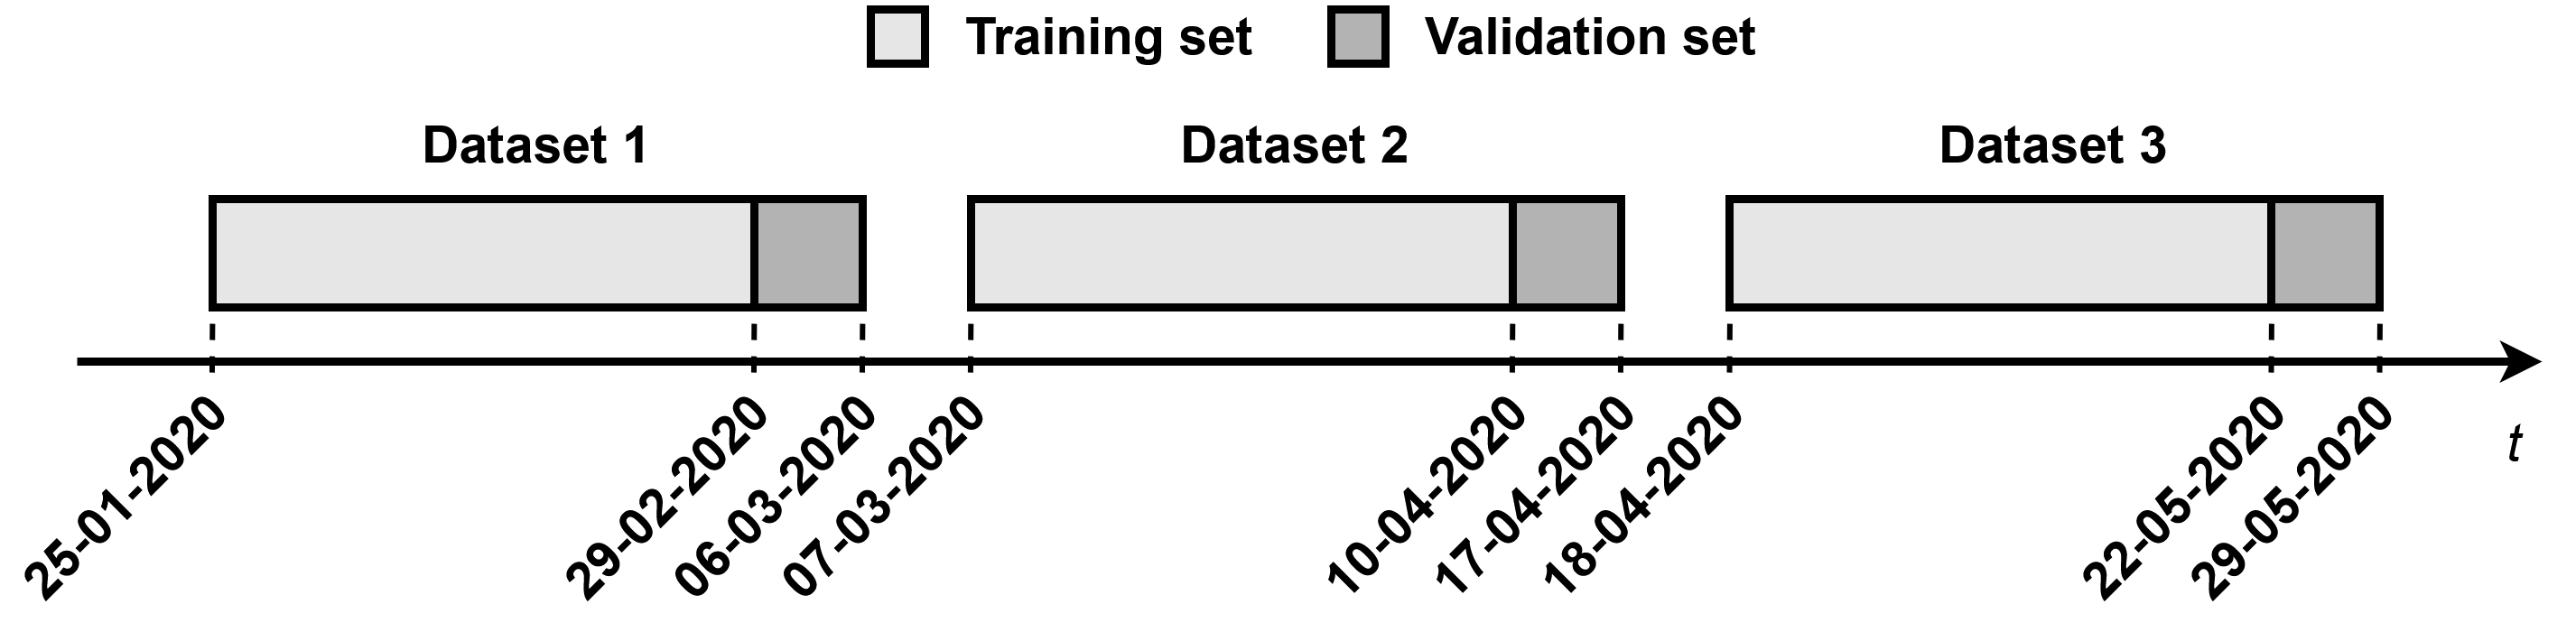
\includegraphics[width=1\textwidth]{Images/hyptun.png}
    \caption{Datasets used for training and validation.}
    \label{hyptun}
    \end{center}
\end{figure}

The process of tuning hyperparators is a long and time consuming process. Although the meaning of each hyperparameter and what it represents in the context of the layer is known, there is no rule dictating which hyperparamters are best for each case. It is an experimental process in which the models must be trained, and validated. The results obtained in the validation data are then compared for different hyperparameter combinations. The combination that presents the best results must be the one selected. All the five models started this phase with layers of 8 units. In models 3, 4 and 5, the initial number of filters of the \ac{1D CNN} layer was also 8 and the kernel\_size used was initially 2. If the models behaved well in the validation set and showed no signs of overfitting or underfitting, the initial values would be maintained. If any of these behaviors were observed in at least one of the datasets, the hyperparameters would be changed, until the model presented the desired behavior for all the three datasets. It was chosen to start with simple architectures and one would only increase the complexity of the architecture (increasing the number of units per layer, for example) if the model did not present all the desired behavior. The increase in the complexity of the model is associated with an increase in its running time, so it was essential to use models as simple as possible. 


Model 1 consists of a input layer with 13 inputs, a \ac{GRU} layer, and a dense layer for the output with 3 units, one for each forecast ((t+5), (t+10) and (t+15)). In \ac{GRU} layers, the hyperparameter that can be changed is the number of Units - A positive integer that represents the dimensionality of the output space. This hyperparameter must be tuned in to find a value for which the system performs well. However, the increase of this value represents an increase in the complexity of the model, which makes it slower.  In this sense, one tested initially a \ac{GRU} layer with 8 units and later a \ac{GRU} with 32 units. Between the two, the structure that presented the best performance was the one with 8 units. In order to avoid overfitting, a drop layer with $p$=0.2 to the \ac{GRU} layer output.Regarding model 2, the structure is relatively similar to model 1 with the difference that it has an \ac{LSTM} layer instead. As in the previous case, it was tested which number of units should be used in the layer, 8 units or 32 units.  Again, the 8-unit layer showed better performance and was therefore chosen. The remaining structure used is similar to model 1. Since the layers of 8 units showed a good behavior for models 0 and 1, this variable was not altered anymore for the remaining models. In the remaining three models, \ac{GRU} and \ac{LSTM} layers of 8 units were always used. In model 3, regarding the \ac{1D CNN} layer, some experiments dictated that a good number of filters - An integer that represents dimensionality of the output space (i.e. the number of output filters in the convolution), to be used could be 8, that is, 8 convolutions are performed that produce the 8 outputs of this layer, but 32 was also tested. The kernel\_size - An integer or tuple/list of a single integer, specifying the length of the 1D convolution window used was 2 units, which means that the output of this layer consists of the result of consecutive convolutions of 2 values, but it was also tested to use a kernel of dimension 10, i.e. convolutions of 10 time-steps that represent 10 minutes, and also of 60 time-steps, i.e. one hour. In the Max pooling layer, a pool\_size of 10 units was used, which means that only the highest value every 10 values is taken into account, as explained in the section \ref{chap3:subsubsec:1dcnn}. In models 4, 5 since they since they are composed of \ac{GRU} and/or \ac{LSTM} layers, combined with a \ac{1D CNN} layer, the same procedure taken into account in models 1, 2 and 3 was put into practice. In Table \ref{tableModels}, a summary of the final models used in the validation process can be found. Factors such as the proposed structure and the number of parameters used are detailed.

\begin{table}[htbp]
  \centering
  \caption{Model specifications.}
    \begin{tabular}{r|cccccccc}
          & \multicolumn{8}{c}{Level 1 Model} \\
    \midrule
    \textbf{Model} & \multicolumn{2}{c}{0} & \multicolumn{2}{c}{1} & \multicolumn{2}{c}{2} & \multicolumn{2}{c}{3} \\
    \midrule
          & \multicolumn{2}{c}{Input (15)} & \multicolumn{2}{c}{Input (15)} & \multicolumn{2}{c}{Input (15)} & \multicolumn{2}{c}{Input (15)} \\
          & \multicolumn{2}{c}{GRU (8)} & \multicolumn{2}{c}{LSTM (8)} & \multicolumn{2}{c}{Conv1D (8, 2)} & \multicolumn{2}{c}{Conv1D (8, 2)} \\
          & \multicolumn{2}{c}{Dropout (0.2)} & \multicolumn{2}{c}{Dropout (0.2)} & \multicolumn{2}{c}{Maxpooling(10)} & \multicolumn{2}{c}{Maxpooling(10)} \\
          & \multicolumn{2}{c}{Dense (3)} & \multicolumn{2}{c}{Dense (3)} & \multicolumn{2}{c}{GRU (8)} & \multicolumn{2}{c}{LSTM (8)} \\
          & \multicolumn{2}{c}{} & \multicolumn{2}{c}{} & \multicolumn{2}{c}{Dropout (0.2)} & \multicolumn{2}{c}{Dropout (0.2)} \\
          & \multicolumn{2}{c}{} & \multicolumn{2}{c}{} & \multicolumn{2}{c}{Dense (3)} & \multicolumn{2}{c}{Dense (3)} \\
    \midrule
    \textbf{Model} & \multicolumn{2}{c}{4} & \multicolumn{2}{c}{5} & \multicolumn{2}{c}{6} & \multicolumn{2}{c}{7} \\
    \midrule
          & \multicolumn{2}{c}{Input (15)} & \multicolumn{2}{c}{Input (15)} & \multicolumn{2}{c}{Input (15)} & \multicolumn{2}{c}{Input (15)} \\
          & \multicolumn{2}{c}{GRU (8)} & \multicolumn{2}{c}{LSTM (8)} & \multicolumn{2}{c}{GRU (8)} & \multicolumn{2}{c}{LSTM (8)} \\
          & \multicolumn{2}{c}{Dropout (0.2)} & \multicolumn{2}{c}{Dropout (0.2)} & \multicolumn{2}{c}{Dropout (0.2)} & \multicolumn{2}{c}{Dropout (0.2)} \\
          & \multicolumn{2}{c}{GRU (8)} & \multicolumn{2}{c}{LSTM (8)} & \multicolumn{2}{c}{LSTM (8)} & \multicolumn{2}{c}{GRU (8)} \\
          & \multicolumn{2}{c}{Dropout (0.2)} & \multicolumn{2}{c}{Dropout (0.2)} & \multicolumn{2}{c}{Dropout (0.2)} & \multicolumn{2}{c}{Dropout (0.2)} \\
          & \multicolumn{2}{c}{Dense (3)} & \multicolumn{2}{c}{Dense (3)} & \multicolumn{2}{c}{Dense (3)} & \multicolumn{2}{c}{Dense (3)} \\
    \midrule
    \textbf{Model} & 0     & 1     & 2     & 3     & 4     & 5     & 6     & 7 \\
    \midrule
    \# inputs & 15    & 15    & 15    & 15    & 15    & 15    & 15    & 15 \\
    \# hidden layers & 2     & 2     & 4     & 4     & 4     & 4     & 4     & 4 \\
    \# hidden nodes & 16    & 16    & 16    & 16    & 16    & 16    & 16    & 16 \\
    \# outputs & 3     & 3     & 3     & 3     & 3     & 3     & 3     & 3 \\
    \end{tabular}%
  \label{tableModels}%
\end{table}%

After defining the structural details of the models to be evaluated, a block cross-validation process was then carried out where Datasets 1, 2 and 3 were trained and validated with a distribution of 75\% training and 25\% validation, i.e. three weeks training and one week of validation. In Appendix D, Tables \ref{table4}, \ref{table5} and \ref{table6}, the reader can find the results of the errors presented in each one of the three datastes. In Table \ref{valres}, the reader may consult the results of the block cross-validation process, which consists of an average of the errors presented in datasets 1, 2 and 3.

\begin{table}[htbp]
  \centering
  \caption{Stage 1 - Block cross-validation results}
       \begin{tabular}{r|cccccccc}
    \toprule
    \multicolumn{1}{c}{} & 0     & 1     & 2     & 3     & 4     & 5     & 6     & 7 \\
    \midrule
    \multicolumn{1}{l|}{\textbf{Non normalized data}} &       &       &       &       &       &       &       &  \\
    \multicolumn{1}{l|}{\textbf{            Validation Score (t+5)      }} &       &       &       &       &       &       &       &  \\
    MSE (E+09)   & \textbf{0.82} & 0.87  & \textbf{0.58} & \textbf{0.67} & 0.90  & 1.18  & 0.91  & 1.02 \\
    RMSE (E+04)   & \textbf{2.84} & 2.92  & \textbf{2.40} & \textbf{2.58} & 2.99  & 3.40  & 2.97  & 3.16 \\
    MAE (E+04)   & \textbf{2.20} & 2.25  & \textbf{1.86} & \textbf{2.06} & 2.30  & 2.62  & 2.30  & 2.45 \\
    \multicolumn{1}{l|}{\textbf{            Validation Score (t+10)               }} &       &       &       &       &       &       &       &  \\
    MSE (E+09)   & \textbf{1.11} & 1.17  & \textbf{0.98} & \textbf{0.99} & 1.20  & 1.42  & 1.16  & 1.28 \\
    RMSE (E+04)   & \textbf{3.30} & 3.39  & \textbf{3.11} & \textbf{3.12} & 3.44  & 3.74  & 3.37  & 3.54 \\
    MAE (E+04)   & \textbf{2.54} & 2.63  & \textbf{2.37} & \textbf{2.43} & 2.65  & 2.89  & 2.59  & 2.76 \\
    \multicolumn{1}{l|}{\textbf{            Validation Score (t+15)               }} &       &       &       &       &       &       &       &  \\
    MSE (E+09)   & \textbf{1.31} & 1.38  & \textbf{1.25} & \textbf{1.24} & 1.43  & 1.63  & 1.38  & 1.51 \\
    RMSE (E+04)   & \textbf{3.58} & 3.68  & \textbf{3.51} & \textbf{3.50} & 3.76  & 4.01  & 3.68  & 3.85 \\
    MAE (E+04)   & \textbf{2.76} & 2.83  & \textbf{2.70} & \textbf{2.71} & 2.89  & 3.09  & 2.82  & 3.01 \\
    \midrule
    \multicolumn{1}{l|}{\textbf{Normalized data}} &       &       &       &       &       &       &       &  \\
    \textbf{Total Validation Score         } &       &       &       &       &       &       &       &  \\
    MSE (E-03)   & \textbf{2.28} & 2.43  & \textbf{2.00} & \textbf{2.11} & 2.47  & 3.03  & 2.36  & 2.56 \\
    RMSE (E-02)   & \textbf{4.70} & 4.84  & \textbf{4.39} & \textbf{4.51} & 4.91  & 5.44  & 4.80  & 5.03 \\
    MAE (E-02)   & \textbf{3.61} & 3.73  & \textbf{3.37} & \textbf{3.51} & 3.77  & 4.20  & 3.69  & 3.90 \\
    \end{tabular}%
  \label{valres}%
\end{table}%



The Table presents the validation \ac{MSE}, \ac{RMSE} and \ac{MAE} for each of the eight models, both for the individual forecast for power available in 5, 10 and 15 minutes, as well as for the overall performance of the model.


It turns out that of all the models tested, the one with the lowest \ac{MSE} and \ac{RMSE}, also presents the lowest \ac{MAE}, Model 2. Since a more detailed comparative study is intended, the three models with the best validation performance, Models 0, 2 and 3, were selected as the three Finalist Models of level 1. These are the three models with the best performance during the block cross-validation procedure. 


(COMENTÁRIOS AOS DADOS)

\section{Stage 2 - Results}\label{chap3:section:stage_2}

\section{Stage 3 - Discussion}\label{chap3:section:stage_3}